\chapter{Introduction}
\label{sec:introduction}

\section{Background and Motivation}
\label{sec:background_motivation}
\begin{German}
    Die Bauindustrie ist einer der grössten Wirtschaftszweige, doch ihre Produktivität stagniert seit Jahrzehnten. In den zwei Jahrzehnten von 1995 bis 2015 wuchs ihre Produktivität nur um 1 \%, weit unter dem globalen Wirtschaftsdurchschnitt von 2.8 \% \cite{barbosaReinventingConstructionRoute2017}. Einer der Gründe ist die geringe Automatisierung.
\end{German}
\begin{English}
    The construction industry is one of the most significant economic sectors, yet its productivity has remained static for several decades. In the period spanning two decades from 1995 to 2015, the observed productivity growth was a mere 1 \%, a figure that falls considerably short of the global economic average of 2.8 \% \cite{barbosaReinventingConstructionRoute2017}. This phenomenon can be attributed, in part, to the limited automation present within the sector.
\end{English}

% Conventional Planning with CAD
\begin{German}
    Zwar wurde die Bauplanung durch den Einsatz von Computer Aided Design (CAD) weitgehend digitalisiert, die Arbeitsschritte blieben jedoch weitgehend die selben \cite{eichlerBIMcertHandbuchGrundlagenwissen2023}. Die konventionelle Planung wurde damit lediglich optimiert. Die Geometrie eines pyhsischen Objekts wird induktiv durch einzelne, meist zweidimensionale Zeichnungen (z.B. Grundriss, Schnitt, Ansicht) abgebildet. Die einzelnen Zeichnungen sind meist isolierte Dateien, die weder geometrisch noch semantisch miteinander verknüpft sind. Änderungen müssen in den betroffenen Zeichnungen manuell vorgenommen werden. \cite{eichlerBIMcertHandbuchGrundlagenwissen2023}
\end{German}

\begin{English}
    Despite the substantial digitalisation of construction planning through the utilisation of computer-aided design (CAD), the fundamental work steps have remained relatively unaltered \cite{eichlerBIMcertHandbuchGrundlagenwissen2023}. Conventional planning was merely optimised. The geometry of a physical object is mapped inductively using individual, usually two-dimensional drawings (e.g. floor plan, section, elevation). The individual drawings are typically isolated files that are neither geometrically nor semantically linked to each other. Alterations require manual adjustments in the affected drawings. \cite{eichlerBIMcertHandbuchGrundlagenwissen2023}
\end{English}

% Model-Based Planning with BIM-Software
\begin{German}
    Erst die Einführung von Building Information Modeling (BIM) ermöglichte eine tiefgreifende Veränderung der Planungsmethodik \cite{eichlerBIMcertHandbuchGrundlagenwissen2023}. Durch BIM können Arbeitsprozesse grundlegend neu strukturiert werden. In der modellbasierten Planung werden neben der geometrischen Form auch semantische Informationen -- etwa zu Materialien oder Kosten -- in ein intelligentes 3D-Modell eingebunden. Verschiedene Fachdisziplinen fügen ihre Inhalte in ein gemeinsames Modell ein, was eine effizientere Zusammenarbeit über den gesamten Lebenszyklus eines Bauwerks ermöglicht. Aus dem Modell lassen sich deduktiv zweidimensionale Zeichnungen ableiten, beispielsweise für den Einsatz auf der Baustelle. Änderungen am Modell werden automatisch in diesen abgeleiteten Zeichnungen aktualisiert. \cite{eichlerBIMcertHandbuchGrundlagenwissen2023}

    Die Einführung von BIM verlief in der Schweiz zunächst zögerlich. Trotz des vorhandenen Produktivitätspotenzials nutzten im Jahr 2021 lediglich 20 \% der Schweizer Bauunternehmen Building Information Modeling \cite{heinrichSchweizImBIMEuropavergleich2022}. Gründe dafür sind die fragmentierte Struktur der Bauwirtschaft sowie ein hoher Preisdruck, wodurch insbesondere kleinere Unternehmen die anfänglich hohen Investitionskosten scheuten \cite{ivanicErfolgreicheEinfuehrungBuilding2020}.
\end{German}

\begin{English}
    The introduction of Building Information Modelling (BIM) enabled a profound change in planning methodology \cite{eichlerBIMcertHandbuchGrundlagenwissen2023}. BIM enables work processes to be restructured fundamentally. In model-based planning, semantic information -- such as that relating to materials or costs -- is integrated into an intelligent 3D model alongside the geometric form. Different specialist disciplines integrate their content into a common model, enabling more efficient collaboration throughout a building's entire life cycle. Two-dimensional drawings can be derived deductively from the model for use on the construction site, for example. Changes to the model are automatically updated in these drawings. \cite{eichlerBIMcertHandbuchGrundlagenwissen2023}

    The introduction of BIM in Switzerland was initially hesitant. Despite the existing productivity potential, only 20 \% of Swiss construction companies were using Building Information Modelling in 2021 \cite{heinrichSchweizImBIMEuropavergleich2022}. This was due to the fragmented structure of the construction industry and high price pressure, which caused smaller companies in particular to shy away from the initially high investment costs \cite{ivanicErfolgreicheEinfuehrungBuilding2020}.
\end{English}

% Telecommunications Planning
\begin{German}
    Die Schweizer Telekommunikationsbranche hat das Potenzial der modellbasierten Planung erkannt. Für die Planung neuer Mobilfunkanlagen auf bestehenden Gebäuden, der sogennanten Rooftop-Standortplanung, soll zukünftig BIM eingesetzt werden. Im Gegensatz zur traditionellen Bauwirtschaft, die sich typischerweise auf grosse, individuelle Bauvorhaben konzentriert, ist die Standortplanung durch ein hohes Projektvolumen mit kleineren, weitgehend standardisierten Infrastruktureingriffen gekennzeichnet. Bereits geringe Effizienzsteigerungen einzelner Arbeitsschritte können sich hier über viele Projekte hinweg aufsummieren. Durch solche Skalenefekte gewinnen automatisierte Planungsprozesse zunehmend an Wirkung.
\end{German}

\begin{English}
    The Swiss telecommunications industry has recognised the potential of model-based planning. In future, BIM is to be used for the planning of new mobile base stations on existing buildings, known as rooftop cell site planning. In contrast to the traditional construction industry, which typically focuses on large, individual construction projects, site planning is characterised by a high project volume with smaller, largely standardised infrastructure interventions. Even minor improvements in the efficiency of individual tasks can result in significant cumulative effects across a large number of projects. As a result of these economies of scale, automated planning processes are becoming increasingly impactful.
\end{English}

% Scan-to-BIM vs Scan-to-GIS
\begin{German}
    Einer dieser automatisierbaren Prozesse ist die digitale Erfassung von Gebäuden mittels Reality Capture. Dabei werden mit Verfahren wie Laserscanning oder Photogrammetrie präzise digitale Abbilder der physischen Umgebung erzeugt. Die daraus gewonnenen digitalen Modelle können als Grundlage für die Planung verwendet werden. Dabei haben sich zwei Ansätze zur Entwicklung digitaler Modelle etabliert:

    \begin{itemize}
        \item \textbf{Scan-to-Mesh:} Bei Scan-to-Mesh wird ein geometrisches Oberflächenmodell (Mesh) erzeugt. Dieses Modell besteht häufig aus tausenden kleinen Dreiecken, die geometrisch nicht logisch gegliedert sind. Es enthält keine semantischen Informationen wie Objektklassen oder Bauteileigenschaften und dient primär der Visualisierung. Während die Generierung relativ schnell erfolgt, ist eine nachträgliche Bearbeitung oder Strukturierung aufwändig. \cite{daiScan2MeshUnstructuredRange2019}
        
        \textit{Analogie (eigene Darstellung): Scan-to-Mesh ist vergleichbar mit dem Einscannen eines Textdokuments als Bild. Der Inhalt ist zwar sichtbar, aber nicht strukturiert oder bearbeitbar.}

        \item \textbf{Scan-to-BIM:} Bei Scan-to-BIM wird ein BIM-Modell für die Nutzung in BIM-Software erzeugt. Dieses Modell besteht aus logisch gegliederten Bauteilen und enthält semantische Informationen. Es dient der detaillierten Planung und Dokumentation von Bauwerken. Die Generierung ist aufwändiger als bei Scan-to-Mesh, da die Modelle eine höhere geometrische Genauigkeit und semantische Struktur aufweisen müssen. \cite{eichlerBIMcertHandbuchGrundlagenwissen2023}
        
        \textit{Analogie (eigene Darstellung): Scan-to-BIM entspricht dem Abtippen des Textdokuments in einem Textbearbeitungsprogramm. Dies ist zwar aufwändiger, erlaubt aber eine nachträgliche Bearbeitbarkeit.} 
    \end{itemize}
\end{German}

\begin{English}
    One such process that has the potential to be automated is the digital recording of buildings using reality capture. This process entails the generation of precise digital images of the physical environment through the utilisation of methodologies such as laser scanning or photogrammetry. The captured digital models provide a reliable data basis for subsequent planning processes. Two principal approaches have been established for the development of digital models:

    \begin{itemize}
        \item \textbf{Scan-to-Mesh:} The Scan-to-mesh process involves the generation of a geometric surface model (mesh). This model frequently comprises thousands of small triangles that are not logically organised geometrically. The absence of semantic information, such as object classes or component properties, is a key feature of this approach, which is primarily employed for the purpose of visualisation. Whilst the initial generation of the data is relatively expeditious, subsequent editing or structuring is time-consuming. \cite{daiScan2MeshUnstructuredRange2019}
        
        \textit{Analogy (author's own): Scan-to-Mesh is comparable to scanning a text document as an image. Despite the content being visible, it is not possible to structure or edit it.}

        \item \textbf{Scan-to-BIM:} Scan-to-BIM facilitates the generation of a BIM model for utilisation within the designated BIM software environment. The model is characterised by the logical organisation of its components and the incorporation of semantic information. The software is utilised for the purpose of meticulous planning and documentation of buildings. The generation process is more intricate than that of Scan-to-Mesh, as the models must possess a higher geometric accuracy and semantic structure. \cite{eichlerBIMcertHandbuchGrundlagenwissen2023}
        
        \textit{Analogy (author's own): Scan-to-BIM is comparable to typing a text document into a word processing program. Despite the increased time investment, this approach facilitates subsequent editing.}
    \end{itemize}
\end{English}

\section{Research Gap}
\label{sec:research_gap}
\begin{German}
    Für die Standortplanung müssen Bauteile nicht nur visualisiert, sondern auch gezielt anpassbar sein. Daher ist ein Scan-to-BIM-Verfahren erforderlich. In den vergangenen Jahren wurde Scan-to-BIM intensiv erforscht und weiterentwickelt \cite{rochaSurveyScantoBIMPractices2021}. Die gefundene Literatur scheint sich primär auf den klassischen Bausektor und die Dokumentation von historischen Gebäuden zu fokusieren. Publikationen, die sich speziell mit Scan-to-BIM für die Standortplanung beschäftigen, konnten keine gefunden werden. Ein möglicher Grund dafür könnte die begrenzte fachliche Relevanz über das Spezialgebiet hinaus sein. Das Anwendungsfled befindet sich in einem spezifischen Schnittstellengebiet zwischen den drei Disziplinen Telekommunikation, Geomatik und Bauwesen (siehe Abb. \ref{fig:intersection}).    
    
    Eine seperate Betrachtung ist aufgrund der individuellen Anforderungen aber sinnvoll. Für die Standortplanung werden keine Innenstrukturen benötigt, und die Fassadengeometrie kann stark vereinfacht dargestellt werden. Im Vergleich zu den Anforderungen der klassischen Baubranche sind die Rahmenbedingungen somit weniger komplex, wodurch eine einfachere Automatisierbarkeit ermöglicht wird -- ein Potenzial, das bislang vor allem in Scan-to-Mesh-Verfahren ausgeschöpft wurde.

    
\end{German}
\begin{English}
    For site planning, components must not only be visualised, but also specifically modifiable. This necessitates the implementation of a Scan-to-BIM workflow. In recent years, Scan-to-BIM has been extensively researched and further developed \cite{rochaSurveyScantoBIMPractices2021}. The extant literature appears to concentrate principally on the conventional construction sector and the documentation of historic buildings. Despite extensive research, no publications specifically addressing site planning were identified. One potential explanation for this phenomenon may be found in the perceived limited professional relevance of the subject beyond the confines of the specialised field. The application area is situated at a particular intersection of three distinct disciplines: telecommunications, geomatics, and construction (see Fig. \ref{fig:intersection}).

    However, a separate consideration is warranted due to the distinct requirements of site planning. The necessity for interior structures is negated, and the geometry of the façade can be represented in a highly simplified form. In comparison to the requirements of the conventional building sector, the framework conditions are therefore less complex, which engenders greater potential for automation -- a potential that has primarily been realised in Scan-to-Mesh approaches.
\end{English}

\begin{figure}[h!]
    \centering
    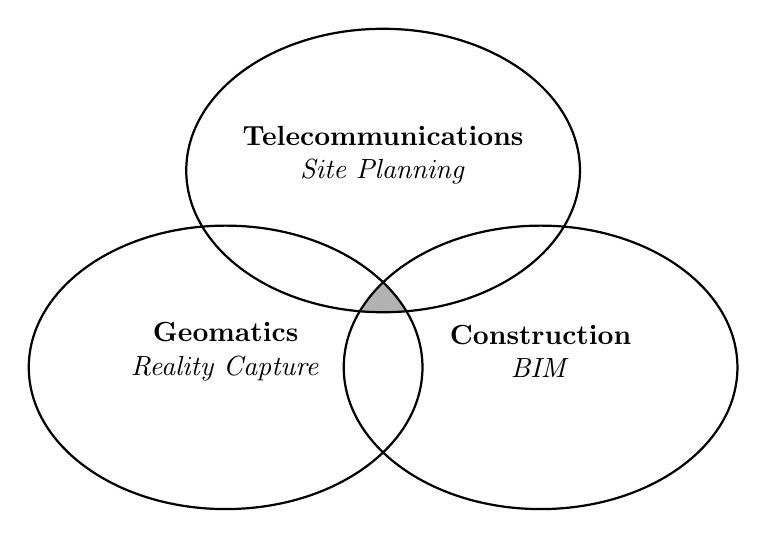
\begin{tikzpicture}[every node/.style={align=center}]

    % Graue Schnittfläche (Intersection)
    \begin{scope}
        \clip (-2,-0.3) ellipse (2.5 and 1.8);
        \clip (2,-0.3) ellipse (2.5 and 1.8);
        \clip (0,2.2) ellipse (2.5 and 1.8);
        \fill[gray!60] (0,0) circle (5);
    \end{scope}

    % Ellipsen
    \draw[thick] (-2,-0.3) ellipse (2.5 and 1.8);  % Geomatics
    \draw[thick] (2,-0.3) ellipse (2.5 and 1.8);   % Construction
    \draw[thick] (0,2.2) ellipse (2.5 and 1.8);    % Telecom

    % Labels in Ellipsen
    \node at (-2,-0.1) {\textbf{Geomatics}\\\textit{Reality Capture}};
    \node at (2,-0.1) {\textbf{Construction}\\\textit{BIM}};
    \node at (0,2.4) {\textbf{Telecommunications}\\\textit{Site Planning}};

    \end{tikzpicture}
    \caption{Intersection of Disciplines}
    \label{fig:intersection}
\end{figure}
    
\section{Research Objectives}
\label{sec:research_objectives}
\begin{German}
    Ziel dieser Arbeit ist die Entwicklung eines automatisieren Scan-to-BIM-Verfahrens für die Standortplanung. Das Verfahren soll eine Punktwolke, also eine Menge räumlicher Messpunkte, einer Gebäudeaussenfläche in ein BIM-Modell überführen. Aus dem Modell soll wiederum ein Baueingabeplan, der den behördlichen Anforderungen genügt, sowie eine Animation abgeleitet werden können. Daraus lassen sich folgende Forschungsfragen ableiten:
\end{German}
\begin{English}
    The aim of this thesis is to develop an automated Scan-to-BIM process for cell site planning. The process is designed to convert a point cloud, i.e. a set of spatial measurement points, of a building exterior into a BIM model. Consequently, it should be feasible to derive a permit drawing that meets regulatory requirements, as well as a visualization, from the model. The following research questions can be derived from this:
\end{English}

    \begin{itemize}
        \item \textbf{Main Question:} How can Scan-to-BIM be automated for telecom rooftop site planning?
        \begin{itemize}
            \item \textbf{Sub-Question 1:} Which steps of Scan-to-BIM can be automated for telecom rooftop site planning?
            \item \textbf{Sub-Question 2:} Which tools enable Scan-to-BIM automation for telecom rooftop site planning?
        \end{itemize}
    \end{itemize}